\PassOptionsToPackage{pdfpagelabels=false}{hyperref} 
\documentclass[final,12pt, times, 5p, twocolumn]{elsarticle}

\usepackage{amsmath}
\usepackage{graphicx}
\graphicspath{ {images/} }

\usepackage[colorinlistoftodos]{todonotes}
\usepackage{url}
\usepackage{hyperref}

%\setlength{\paperheight}{11in}
%\setlength\fboxsep{0pt}
%\setlength\fboxrule{0.5pt}

\usepackage[brazilian]{babel}
\usepackage[utf8x]{inputenc}

\usepackage[T1]{fontenc}
\usepackage{amssymb}

\selectlanguage{brazilian}

\begin{document}

\begin{frontmatter}

\title{Bduíno - Um dispositivo para a captura de dados do contexto urbano para o uso da bicicleta.}

\author[ant]{Antonio Fernando Santos Ladeia}
\author[pab] {Orientador(a): Pablo Vieira Florentino}

\address[ant]{Instituto Federal da Bahia}
\address[pab]{Instituto Federal da Bahia}

\begin{abstract}
%% Text of abstract

\end{abstract}

\begin{keyword}
Microcontroller \sep Ambiental Data \sep Bicycle \sep Open Hardware \sep Open Source \sep Embedded Systems
\end{keyword}

\end{frontmatter}

\section{Introdução}

Enquanto os espaços para automóveis apenas aumentam no contexto atual, outros modais, não recebem a devida atenção das autoridades competentes, somando-se a isso uma possível falta de atratividade para o uso desses modais.

Questões ambientais e urbanas podem ser fatores determinantes para a popularização do uso de outros modais, como a bicicleta, por isso este trabalho tenta posicionar-se de forma a descobrir possíveis fatores que podem afastar ou trazer novos usuários para este modal.

Nesse intento a aplicação Bduíno, foi pensada desde a sua concepção para ser uma solução capaz de responder alguma dessas questões, além de basear-se em pilares fundamentais como o desenvolvimento livre e replicável, a adaptação do projeto para necessidades específicas, dando o direito ao usuário final aprender e compartilhar com a solução. 

\subsection{Justificativa}

A mobilidade urbana é um ponto de ampla discussão e impacto na sociedade atual. Os espaços reservados aos automóveis multiplicam-se, tomando o espaço de transportes coletivos e não motorizados, como calçadas ou bicicletas. Com a facilidade de acesso ao financiamento e a isenção de impostos, mais e mais pessoas ocupam as ruas com seus carros particulares,  dificultando o trânsito  e prejudicando a vida da grande maioria.

Na prática, não existem políticas governamentais de que possuam como objetivo legitimar outras formas de mobilidade, como a bicicleta, como um modal de transporte reconhecido, promovendo o seu uso e conscientizando condutores de veículos motorizados sobre as leis de trânsito para um compartilhamento pacífico e amigável das ruas. 

Este contexto gera um ambiente hostil para os usuários de bicicleta e desencorajador para aqueles que gostariam de adotar este modal de locomoção nas cidades. Faltam iniciativas e dados que melhor detalhem e quantifiquem este contexto adverso como:
\begin{itemize}

  \item Altas velocidades nas ruas e avenidas
  \item Falta de sinalização
  \item Ruas arborizadas
  \item Distância entre veículos motorizados e bicicletas.

\end{itemize}

\subsection{Objetivos}

Este trabalho possui como objetivo principal a captura de informações reais e detalhadas relativas ao ambiente das ruas a partir do uso de bicicletas, para melhor entender os fatores que fazem as ruas dos grandes centros urbanos tão hostis e desmotivadores deste meio de transporte. 

Busca-se, assim, tratar tanto das questões ambientais como das questões de tráfego urbano e das condições, favoráveis, ou não, para o uso da bicicleta.

Nesta mesma linha de raciocínio, temos como objetivos secundários:

\begin{itemize}

  \item Mapear espacialmente/geograficamente os dados coletados, no sentido de indicar os trechos com condições mais favoráveis ou menos atrativos;
  \item Oferecer subsídios para políticas de adequação do espaço;
  \item A observação da legitimação das políticas públicas de transito por parte de motoristas e ciclistas, avaliando esta relação nas práticas de uso das pistas em séries periódicas. \ldots

\end{itemize}

O trabalho está organizado em seções e será apresentado na seguinte ordem:

\begin{enumerate}	
    \item Na seção 2 será mostrado apresentado o referencial teórico. 
    \item Na seção 3 serão mostrados os trabalhos correlatos.
    \item Na seção 4 será detalhado a metodologia utilizada no desenvolvimento deste trabalho.
    \item Na seção 5 será discutida as tecnologias adotadas nesta solução.
    \item Na seção 6 será apresentada a solução proposta por este trabalho.
    \item Na seção 7 será apresentado os testes e resultados obtidos com a solução.
    \item Na seção 8 será apresentada a conclusão do trabalho.
    \item Na seção 9 será apresentada as idéias para o futuro do projeto.
\end{enumerate}

\section{Referencial teórico}

Para entender o contexto onde o trabalho está situado, é importante conhecer alguns conceitos em que ele se fundamenta, por isso, esta sessão tem por objetivo pautar os trabalhos similares e os que serviram de referencial para o mesmo.

\subsection{Software Livre}

O conceito de Software Livre~\cite{softwareLivre} nasce com o projeto GNU~\cite{GNU}. O Software Livre possui enraizada a filosofia de ser um movimento social ao invés de apenas uma decisão técnica. Ela é muito mais que apenas código aberto, ela é uma posição política e filosófica que se opõe ao software proprietário na medida em que o conhecimento gerado com o software proprietário é fechado a poucas pessoas.

Para um \texttt{software} ser considerado livre, ele precisa seguir quatro liberdades, que são os pilares do movimento Software Livre, aqui traduzidas livremente:

\begin{itemize}
  \item A liberdade de executar o programa, para qualquer propósito (liberdade nº 0)
  \item A liberdade de estudar como o programa funciona e adaptá-lo para as suas necessidades (liberdade nº 1). O acesso ao código-fonte é um pré-requisito para esta liberdade.
  \item A liberdade de redistribuir cópias de modo que você possa ajudar ao seu próximo (liberdade nº 2).
  \item A liberdade de aperfeiçoar o programa, e liberar os seus aperfeiçoamentos, de modo que toda a comunidade se beneficie deles (liberdade nº 3). O acesso ao código-fonte é um pré-requisito para esta liberdade.
\end{itemize}

\subsection{Hardware Open-source}

O conceito de Hardware Open-source surgiu apoiado no conceito de Software Open-source, mas assim como este, não se restringiu apenas a parte técnica dos dispositivos físicos. O Hardware Open-source extrapolou as fronteiras da computação e engenharia e hoje temos vários projetos de \textit{Hardware Open-source} dentro da arquitetura e do urbanismo, como os projetos \textit{Wikihouse} e o Arc e Tec, na criação de máquinas,como o \textit{Open Source Ecology}, entre outros. Alguns projetos interessantes são citados a seguir:

\subsubsection{Máquinas livres}

\begin{figure}[ht!]
\centering
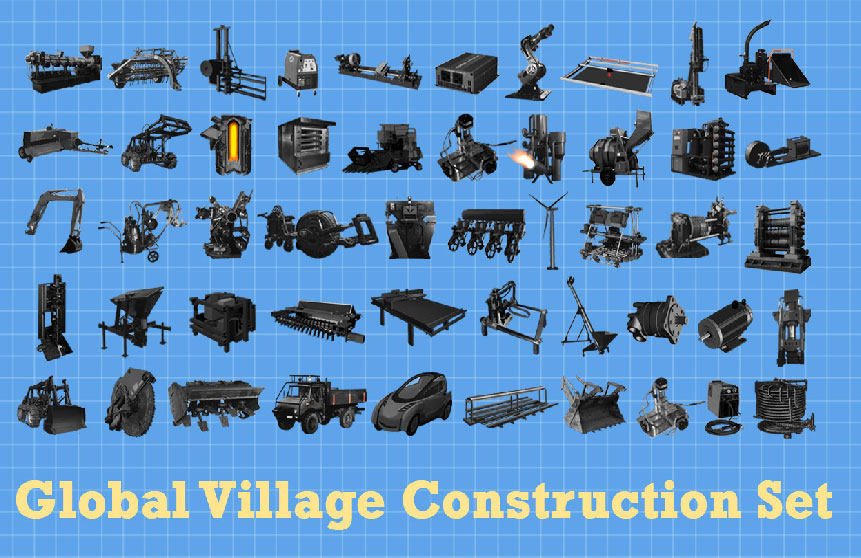
\includegraphics[width=0.5\textwidth]{gvcs.jpg}
\caption{\label{fig:gvcs}Kit de construção de vilas}
\end{figure}

O site Open Source Ecology \cite{Open Source Ecology} possui um projeto chamado \textit{Machines: Global Village Construction Set} \cite{Machines: Global Village Construction Set}, que consiste em uma coleção de projetos open source criados com o intuito de liberar o conhecimento sobre a fabricação de máquinas industriais  para construir uma pequena e sustentável civilização com confortos modernos.

O projeto cria trambém ferramentas que podem ser usadas para replicar as próprias ferramentas, fazendo com que elas possam ser facilmente difundidas, replicadas e melhoradas, resultando, no final num projeto orçado apenas em uma fração do projeto original. O projeto também possui como objetivo a qualidade do material criado, o desempenho na produção das mesmas, a capacidade de replicação e a eficiência de cada uma, tanto para as construções, quanto as ferramentas. O projeto trabalha fortemente com a idéia da construção de artefatos que necessitem de baixa manutenção, possuam a produção escalável e possam ser usados de forma social para mudar os hábitos das pessoas. O projeto ainda não foi finalizado, no site é possível acompanhar a concepção e produção de cada ferramenta individual, além de uma comparação de custos entre pesquisas, protótipos e as versões comerciais da mesma.

\subsubsection{Arquitetura livre}

A arquitetura livre pode ser encontrada nos sites Wikihouse \cite{Wikihouse} e no site Arc e Tec \cite{Arc e Tec}, nestes sites são compartilhados projetos de arquitetura,urbanismo e design \textit{open source}.

A WikiHouse é uma fundação que mantém uma plataforma que abriga um sistema de construção de código aberto. Uma área comum para projetos de casas de alto desempenho, baixo consumo de energia que podem ser personalizadas, digitalmente fabricados e auto-montado. A WikiHouse está colaborando para criar e colocar ferramentas e conhecimentos sustentáveis de design para nas mãos de todos.

Estes projetos mostram como o crescimento das idéias do hardware livre estão propagando-se para além das máquinas e adentrando outras áreas, como é o caso da arquitetura.

\subsection{Microcontroladores}

Os microcontroladores são microprocessadores que podem ser programados para funções específicas. Em geral, eles são usados para controlar circuitos e, por isso, são comumente encontrados dentro de outros dispositivos, sendo conhecidos como "controladores embutidos". A estrutura interna de um microcontrolador apresenta um processador bem como circuitos de memória e periféricos de entrada e saída.

Cerca de 50\% dos microcontroladores vendidos são controladores "simples", outros 20\% são processadores de sinais digitais (DSPs) mais especializados. Os microcontroladores podem ser encontrados em praticamente todos os dispositivos eletrônicos digitais que nos cercam: teclado do computador, dentro do monitor, disco rígido, relógio de pulso, rádio relógio, máquinas de lavar, forno de micro-ondas, telefone, etc. Certamente eles foram tão ou mais importantes para a revolução dos produtos eletrônicos que os computadores. Eles permitiram a evolução de equipamentos que há anos não evoluíam  como os motores a combustão, que agora com o novo controle eletrônico podem funcionar com sistema biocombustível, poluindo menos e as máquinas fotográficas, que migraram de processos químico/mecânico a circuitos com microcontroladores+Sensores Digitais+Memória.

Com freqüências de {\it clock} de poucos {\it MHz (Megahertz)} ou talvez menos, os microcontroladores operam a uma freqüência muito baixa se comparados com os microprocessadores atuais, no entanto são adequados para a maioria das aplicações. O seu consumo em geral é relativamente pequeno, normalmente na casa dos {\it miliwatts} e possuem geralmente habilidade para entrar em modo de espera ({\it Sleep} ou {\it Wait}) aguardando por uma interrupção ou evento externo, como por exemplo, o acionamento de uma tecla, ou um sinal que chega via uma interface de dados. O consumo destes microcontroladores em modo de espera pode chegar à casa dos {\it nanowatts}, tornando-os ideais para aplicações onde a exigência de baixo consumo de energia é um fator decisivo para o sucesso do projeto.

Os microcontroladores se diferenciam dos processadores, pois além dos componentes lógicos e aritméticos usuais de um microprocessador de uso geral, o microcontrolador integra elementos adicionais em sua estrutura interna, como memória de leitura e escrita para armazenamento de dados, memória somente de leitura para armazenamento de programas, EEPROM para armazenamento permanente de dados, dispositivos periféricos como conversores analógico/digitais (ADC), conversores digitais/analógicos (DAC), Portas de entrada e Saída digitais(I/O) para propósito geral.

Um microcontrolador geralmente é pequeno e barato\cite{marshallbrainmicrocontrolador}. Os componentes são escolhidos para minimizar o tamanho e serem os mais econômicos possíveis. Um microcontrolador geralmente é feito para ser mais robusto de alguma forma. O microcontrolador que controla um motor de carro, por exemplo, tem que trabalhar em temperaturas extremas que um computador normalmente não suporta. Um microcontrolador de carro no Alaska tem que funcionar bem em temperaturas de -34ºC, enquanto o mesmo microcontrolador no Rio de Janeiro pode ter de operar a 42ºC. Quando se adiciona o calor que é gerado naturalmente pelo motor, a temperatura pode atingir de 65 a 80ºC no compartimento do motor. Por outro lado, um microcontrolador embutido dentro de um VCR não precisa ser tão resistente assim \cite{marshallbrainmicrocontrolador}.

\subsubsection{Arduíno}

O Arduíno \cite{Arduino} é uma família de ferramentas e placas de circuito integrados utilizadas para prototipagem de circuitos. Ele é utilizado para fazer com que computadores possam controlar mais dispositivos eletrônicos existentes no mundo físico além dos próprios computadores pessoais. Ele é uma plataforma física \textit{open source} de computação baseada num microcontrolador, e alguns outros componentes atrelados a uma interface de comunicação com outros dispositivos através de pinos digitais e analógicos. 

O Arduíno conta ainda com um ambiente de desenvolvimento integrado para escrever, testar, compilar e embarcar os softwares para a placa \cite{arduinoworkshop}.

\subsection{Raspberry Pi}

O Raspberry Pi é "um computador em uma placa" do tamanho aproximado de um cartão de crédito. Ele possui um processador single core com barramento de 700 MHZ, uma memória ram de 512MB \cite{programandoraspberrypi}. O raspberry Py conta ainda com um slot para um cartão SD (Secure Digital) com capacidade de 8GB e classe 10, onde estarão armazenados o sistema operacional que controla o Raspberry Pi, os \textit{scripts} da aplicação responsáveis pela comunicação, recebimento, tratamento e armazenamento dos dados vindos do Arduíno.

O Raspberry Pi também possui pinos digitais que poderiam ser utilizados para realizar algumas medições, mas a corrente de alimentação do Rapberry Pi é menor que a necessária para alimentar os dispositivos.

O Raspberry funcionará neste projeto como dispositivo principal, cabendo a ele o papel de receber os dados através de uma conexão serial, tratar os dados e persisti-los. Caberá também ao Raspberry Pi a tarefa posterior ao uso da bicicleta, a transmissão de dados capturados para a plataforma web desenvolvida.

No Raspberry Pi a linguagem de programação escolhida foi o Python, por ser uma linguagem de script que possui uma gama de bibliotecas para diversas funções já disponíveis, o Python também possui ótima compatibilidade com o dispositivo, já vindo pré instalada na distribuição GNU/Linux adotada, o Raspbian. Foi utilizado também um pequeno script em linguagem shell para inicializar os scripts em Python durante a inicialização do sistema. 

\begin{figure}[ht!]
\centering
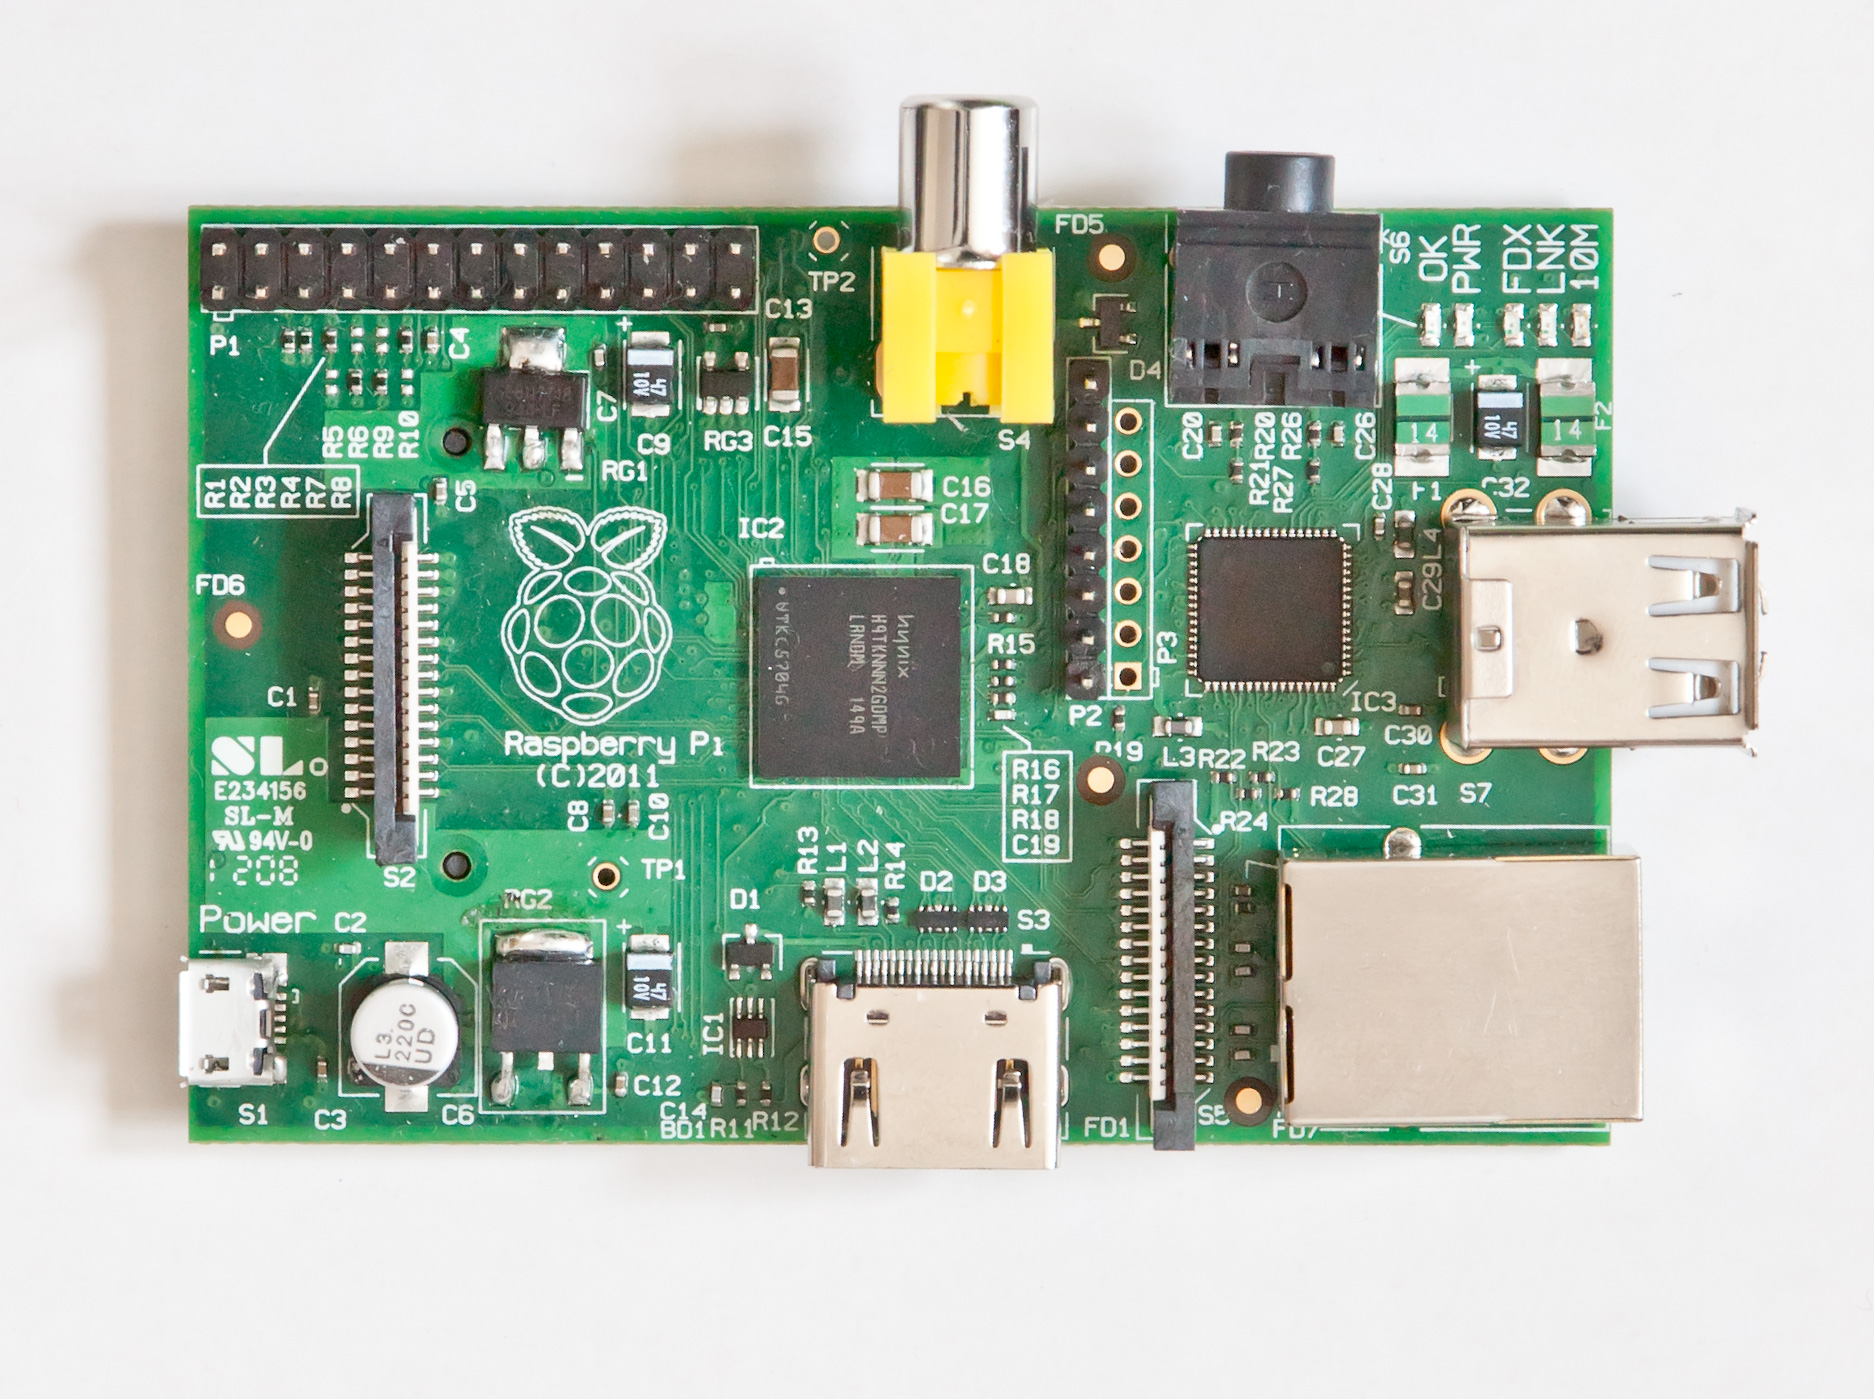
\includegraphics[width=0.5\textwidth]{pi.jpg}
\caption{\label{fig:pi}Raspberry Pi}
\end{figure}

\subsection{Sistemas embarcados}

Um sistema embarcado é um sistema microprocessado no qual o computador é completamente encapsulado ou dedicado ao dispositivo ou sistema que ele controla. Diferentemente de computadores de propósito geral, como o computador pessoal, um sistema embarcado realiza um conjunto de tarefas predefinidas, geralmente com requisitos específicos. Já que o sistema é dedicado a tarefas específicas, através de engenharia pode-se otimizar o projeto reduzindo tamanho, recursos computacionais e custo do produto.

Em geral tais sistemas não podem ter sua funcionalidade alterada durante o uso. Caso queira-se modificar o propósito é necessário reprogramar todo o sistema.

Sistemas como PDAs são geralmente considerados sistemas embarcados pela natureza de seu hardware, apesar de serem muito mais flexíveis em termos de software. Fisicamente, os sistemas embarcados vão desde MP3 players a semáforos.

\subsection{Energia solar}

Energia solar é um termo que se refere à energia proveniente da luz e do calor do Sol. É utilizada por meio de diferentes tecnologias em constante evolução, como o aquecimento solar, a energia solar fotovoltaica , a energia heliotérmica, a arquitetura solar e a fotossíntese artificial \cite{SolarFuel}.

Tecnologias solares são amplamente caracterizadas como ativas ou passivas, dependendo da forma como captura, converte e distribui a energia solar. Entre as técnicas solares ativas estão o uso de painéis fotovoltaicos e coletores solares térmicos das usinas heliotérmicas, para aproveitar a energia. Entre as técnicas solares passivas estão a orientação de um edifício para o Sol, a seleção de materiais com massa térmica favorável ou propriedades translúcidas e projetar espaços que façam o ar circular naturalmente.

No seu movimento de translação ao redor do Sol, a Terra recebe 1 410 W/m² de energia, medição feita numa superfície normal (em ângulo reto) com o Sol. Disso, aproximadamente 19\% é absorvido pela atmosfera e 35\% é reflectido pelas nuvens. Ao passar pela atmosfera terrestre, a maior parte da energia solar está na forma de luz visível e luz ultravioleta. As plantas utilizam diretamente essa energia no processo de fotossíntese. Nós usamos essa energia quando queimamos lenha ou combustíveis minerais. Existem técnicas experimentais para criar combustível a partir da absorção da luz solar em uma reação química de modo similar à fotossíntese vegetal - mas sem a presença destes organismos. A radiação solar, juntamente com outros recursos secundários de alimentação, tal como a energia eólica e das ondas, hidro-electricidade e biomassa, são responsáveis por grande parte da energia renovável disponível na terra. Apenas uma minúscula fracção da energia solar disponível é utilizada.

Em 2011, a Agência Internacional de Energia disse que "o desenvolvimento de tecnologias de fontes de energia solar acessíveis, inesgotáveis e limpas terá enormes benefícios a longo prazo. Ele vai aumentar a segurança energética dos países através da dependência de um recurso endógeno, inesgotável e, principalmente, independente de importação, o que aumentará a sustentabilidade, reduzirá a poluição, reduzirá os custos de mitigação das mudanças climáticas e manterá os preços dos combustíveis fósseis mais baixos. Estas vantagens são globais. Sendo assim, entre os custos adicionais dos incentivos para a implantação precoce dessa tecnologia devem ser considerados investimentos em aprendizagem; que deve ser gasto com sabedoria e precisam ser amplamente compartilhados" \cite{artigoenergiasolar}.

\section{Trabalhos correlatos}

Abaixo são apontados alguns trabalhos que tangem, em maior ou menor grau, algumas das funcionalidades deste projeto, ou serviram de inspiração na concepção e no andamento deste trabalho.

\subsection{Sensorium}

\begin{figure}[ht!]
\centering
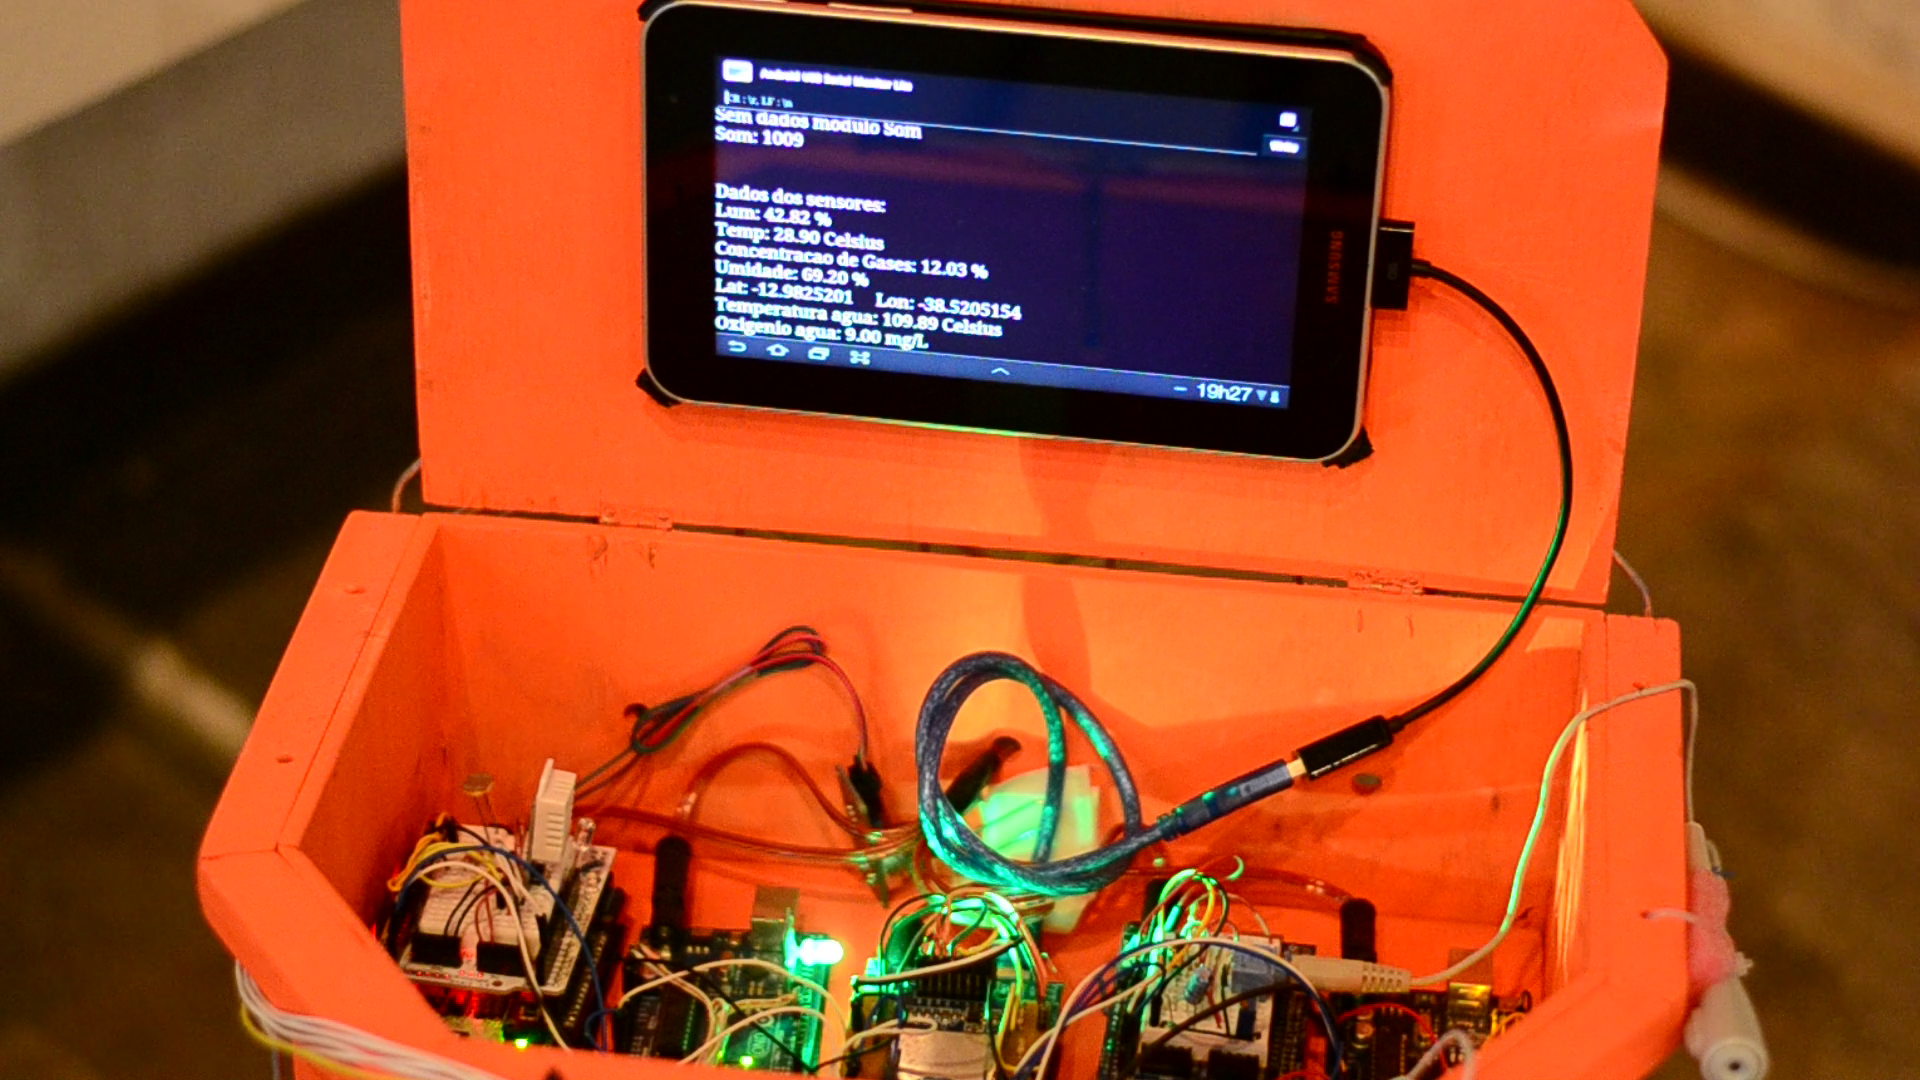
\includegraphics[width=0.5\textwidth]{sensorium.png}
\caption{\label{fig:sensorium.png}Sensorium}
\end{figure}

Sensorium é um projeto de arte, tecnologia e inovação criado pelo grupo de pesquisa Ecoarte – IHAC/Universidade Federal da Bahia - UFBA que consiste na criação de um dispositivo móvel com o uso de sensores para fazer a interação com o ambiente. O projeto Sensorium foi dividido em 4 fases, sendo elas a criação do dispositivo, uma \textit{performance} com ação da comunidade, a visualização dos dados coletados e a exposição do projeto artístico e seus processos \cite{artigosensorium}.

A criação do dispositivo envolveu prioritariamente soluções livres, tanto de \textit{hardware} quanto de \textit{software}, a facilidade operacional do dispositivo, a geração e a leitura dos dados obtidos por pessoas não ligadas a área técnica/tecnológica.

Para tanto, o protótipo foi construído com o microcontrolador arduino, utilizando os sensores de temperatura do ar e da água, umidade relativa do ar, salinidade, níveis de intensidades sonoras, níveis de CO2, GPS e Ultra violeta.

\subsection{The Copenhagen Wheel}

\begin{figure}[ht!]
\centering
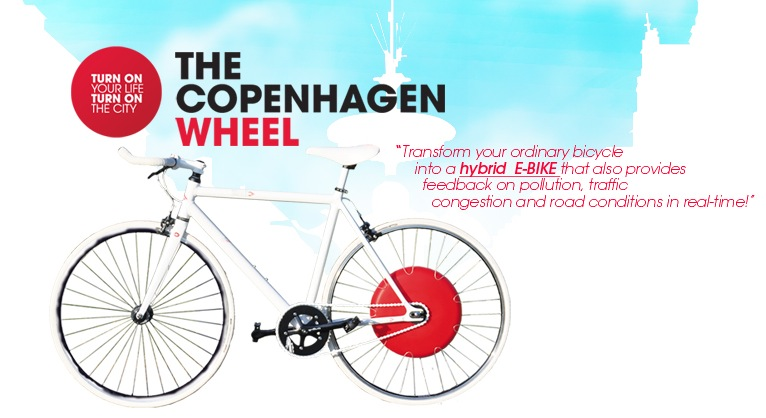
\includegraphics[width=0.5\textwidth]{tcw.jpg}
\caption{\label{fig:tcw.jpg}The Copenhagen Wheel}
\end{figure}

Este projeto foi criado por um grupo no Instituto de tecnologia de Massachucets (\textit{Massachucets Institute of Thecnologic}) ou MIT no ano de 2005 tem como objetivo transformar biciletas comuns em bicicletas eletrônicas, ou e-bikes \cite{e-bikes}.

O projeto usa o \textit{smartphone} para controlar o dispositivo que está acoplado à bicicleta e mapeia os níveis de poluição, congestionamento do tráfego e as condicões da estrada em tempo real \cite{artigotcw}. 
Enquanto a bicicleta é usada, os sensores da bicicleta capturaram informações sobre suas preferências pessoais de ciclismo, como quanto esforço é posto nisso, quantas calorias foram queimadas e etc assim como as informações sobre o ambiente, incluindo quantidade de monóxido de carbono, óxido de nitrogênio (NOx), níveis de ruído, temperatura ambiental e umidade relativa.

\section{Metodologia}

Primeiramente foram analisados os resultados de uma pesquisa sobre o uso da bicicleta  e fatores relativos, realizada no ano de 2012 entre pessoas de diferentes perfis e majoritariamente participantes de grupos de usuários de bicicletas em Salvador \cite{pesquisamobilidade}.

Analisadas essas informações, foram definidos diversos aspectos que poderiam ser aferidos através de um dispositivo eletrônico a ser anexado a uma bicicleta, afim de medir alguns destes fatores.

Serão analisados fatores ambientais como:

\begin{itemize}

  \item Temperatura do ar.
  \item Umidade do ar.
  \item Luminosidade.
  \item Nível de ruído.

\end{itemize}

assim como fatores urbanos:

\begin{itemize}

  \item Nível de trepidação da pista.
  \item Distância em que outros veículos motorizados passam pelo usuário de bicicleta.
  \item Velocidade em que outros veículos motorizados passam pelo usuário.

\end{itemize}

\subsection{Criação de dispositivo}

A criação do dispositivo foi feita num processo de melhoria contínua, utilizando-se de incrementos funcionais aplicados ao dispositivo que visam a criação de aplicações de testes, a integração dessas aplicações e as correções dos erros encontrados durante o processo de desenvolvimento do sistema.

\subsubsection{Primeira fase}

A primeira fase é composta de duas aplicações que executam em dois ambientes heterogênos, a saber, o Arduíno, um sistema embarcado, e o Rapberry Pi, um computador diminuto. Cada aplicação desse sistema, funciona de forma independente da outra devendo apenas executar uma pequena fração da aplicação total, para testar a sua viabilidade.

A primeira aplicação desenvolvida é um script que executará na plataforma Raspberry Pi, este script ficará encarregado de manter uma comunicação serial e receber os dados que por ela chegarem, armazenando-os em um arquivo texto simples. A evolução dessa aplicação se dará com a mesma inicializando juntamente com o Sistema operacional do Raspberry Pi, afim de começar a coletar os dados automaticamente, além de gravar os dados recebidos de uma forma estruturada em um banco de dados relacional.

A segunda aplicação é uma aplicação embarcada que executará na plataforma Arduíno. Essa aplicação será responsável pela execução de algumas tarefas, como:

\begin{itemize}

  \item Iniciar uma comunicação serial.
  \item Coletar os dados dos sensores e atuadores nele conectados.
  \item Enviar os dados coletados através da conexão serial criada.

\end{itemize}

\subsection{Testes de rua}

Após a etapa da criação do dispositivo, será iniciada a fase de testes com o mesmo, afim de capturar e remover possíveis falhas encontradas.

Na fase seguinte, serão coletados os primeiros dados através de parcerias com ciclistas locais.

\section{Soluções adotadas}

O desenvolvimento do dispositivo se dará através da plataforma  de \textit{hardware} \textit{Open-source}, Arduíno, juntando se a isso os sensores necessários para a checagem das informações ambientais e urbanas. Apartir desse conjunto, os dados serão capturados, sem nenhum tipo de tratamento, e serão enviados, através de uma conexão serial\cite{Conexao Serial}, para outro dispositivo, com mais capacidade de processamento, mas ainda sim portável, o RaspBerry Pi\cite{Raspberry Pi}, onde os dados serão então tratados e armazenados para posterior utilização.

Os dados capturados serão armazenados em um contexto espacial (geolocalizados) e temporal.

\subsection{Microcontrolador}

O desenvolvimento do dispositivo será feito com o Arduíno Mega 1650 por este modelo possuir melhor custo/benefício em comparação aos outros modelos da plataforma. 

Ele possui uma memória maior, possibilitando, assim, maior flexibilidade na captura de maiores volumes de dados sem comprometer o desempenho do dispositivo, além de contar com um número maior de portas digitais e analógicas possibilitando, que o dispositivo seja flexível para receber novos sensores e capturar dados diferentes de acordo com a necessidade local.

O Arduino mega 2560 é uma placa de microcontrolador baseado no ATmega2560. Ele tem 54 pinos digitais de entrada / saída (dos quais 15 podem ser usados como saídas PWM), 16 entradas analógicas, 4 UARTs (portas seriais de hardware), um oscilador de cristal de 16 MHz, uma conexão USB, um conector fonte de energia e um botão de reinicialização. Este conjunto contém tudo o que é necessário para apoiar o microcontrolador, basta conectá-lo a um computador com um cabo USB ou ligá-lo com um adaptador AC/DC. O mega é compatível com a maioria dos \textit{shields}, placas de expansão de funcionalidades, projetados para o Arduino Duemilanove ou Uno, as versões mais comuns encontradas.

\begin{figure}[ht!]
\centering
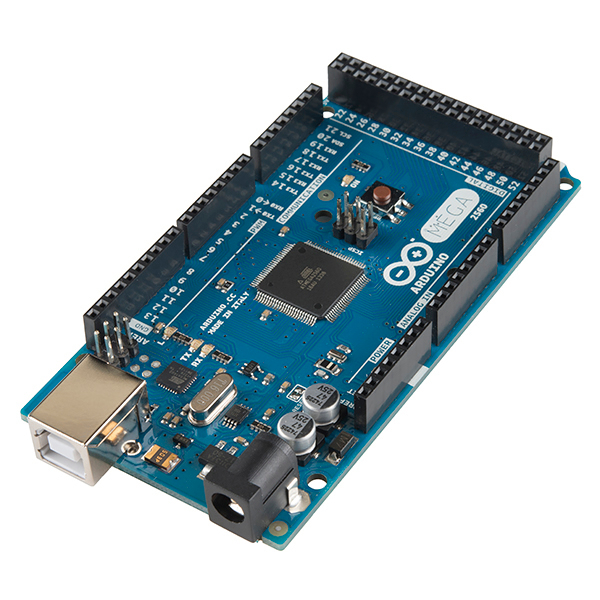
\includegraphics[width=0.5\textwidth]{mega.jpg}
\caption{\label{fig:mega}Arduíno mega}
\end{figure}

\subsection{Python}

O Python é uma linguagem de programação de propósito geral, amplamente utilizada e de alto nível. A sua filosofia de design realça a legibilidade do código, e sua sintaxe permite que os programadores possam expressar conceitos em menos linhas de código do que seria possível em línguagens tais como C ++ ou Java. A linguagem fornece construções destinados a permitir programas claros, tanto numa escala pequena ou grande.

Python suporta múltiplos paradigmas de programação, incluindo, a programação imperativa, funcional, orientação a objetos ou procedural. Ela possui um sistema de tipagem dinâmica, gerenciamento automático de memória e tem um conjunto grande e abrangente da biblioteca padrão \cite{pythonsite}.

Além da biblioteca padrão do Python, será utilizada também a bilboteca PySerial, responsável por abstrair todo o protocolo de comunicação serial.

\subsection{Raspbian}

O Raspbian é uma versão não-oficial do Debian Wheezy com configurações de compilação ajustadas para produzir código otimizado "\textit{hard float}", possuindo por exemplo, um chip físico para tratar dos números de ponto flutuante, que será executado no Raspberry Pi. Isso fornece um desempenho significativamente mais rápido para aplicações que fazem uso pesado de operações aritméticas de ponto flutuante. Todas as outras aplicações também vão ganhar algum desempenho através do uso de instruções avançados da CPU ARMv6 no Raspberry Pi.

Embora o Raspbian seja construído principalmente através de esforços de Mike Thompson (mpthompson) e Peter Green (plugwash), ele também se beneficiou muito com o apoio entusiástico dos membros da comunidade do Raspberry Pi que desejam obter o máximo desempenho do seu dispositivo.

Por se tratar de um sistema operacional baseado em GNU/Linux, é possível o uso de recursos avançados do sistema operacional, por exemplo, se fez necessário a alteraração de um script de inicialização do sistema operacional para que a aplicação que consome os dados que chegam pela porta serial fosse inicializada junto com o sistema, bastanto apenas que houvesse alimentação elétrica para o sistema começar a funcionar, e este recurso estava facilmente disponível neste sistema operacional, da mesma forma que em um sistema operacional convencional.

\subsection{Alimentação elétrica}

A alimentação deste conjunto formado pelo Arduíno com seus sensores e o Raspberry Pi, é feita através de uma bateria com capacidade nominal de 30000 MAH, e capacidade real de 16000 MAH.

Esta bateria pode ser alimentada por uma fotocélula ou por energia elétrica convencional. Neste projeto utilizamos a recarga solar enquanto o ciclista se locomove em ambientes iluminados, com isso o projeto ganha maior autonomia, e ainda conseguimos usar uma tecnologia verde\cite{tecnologia verde} não poluente, e que se utiliza de uma fonte renovável.

\begin{figure}[ht!]
\centering
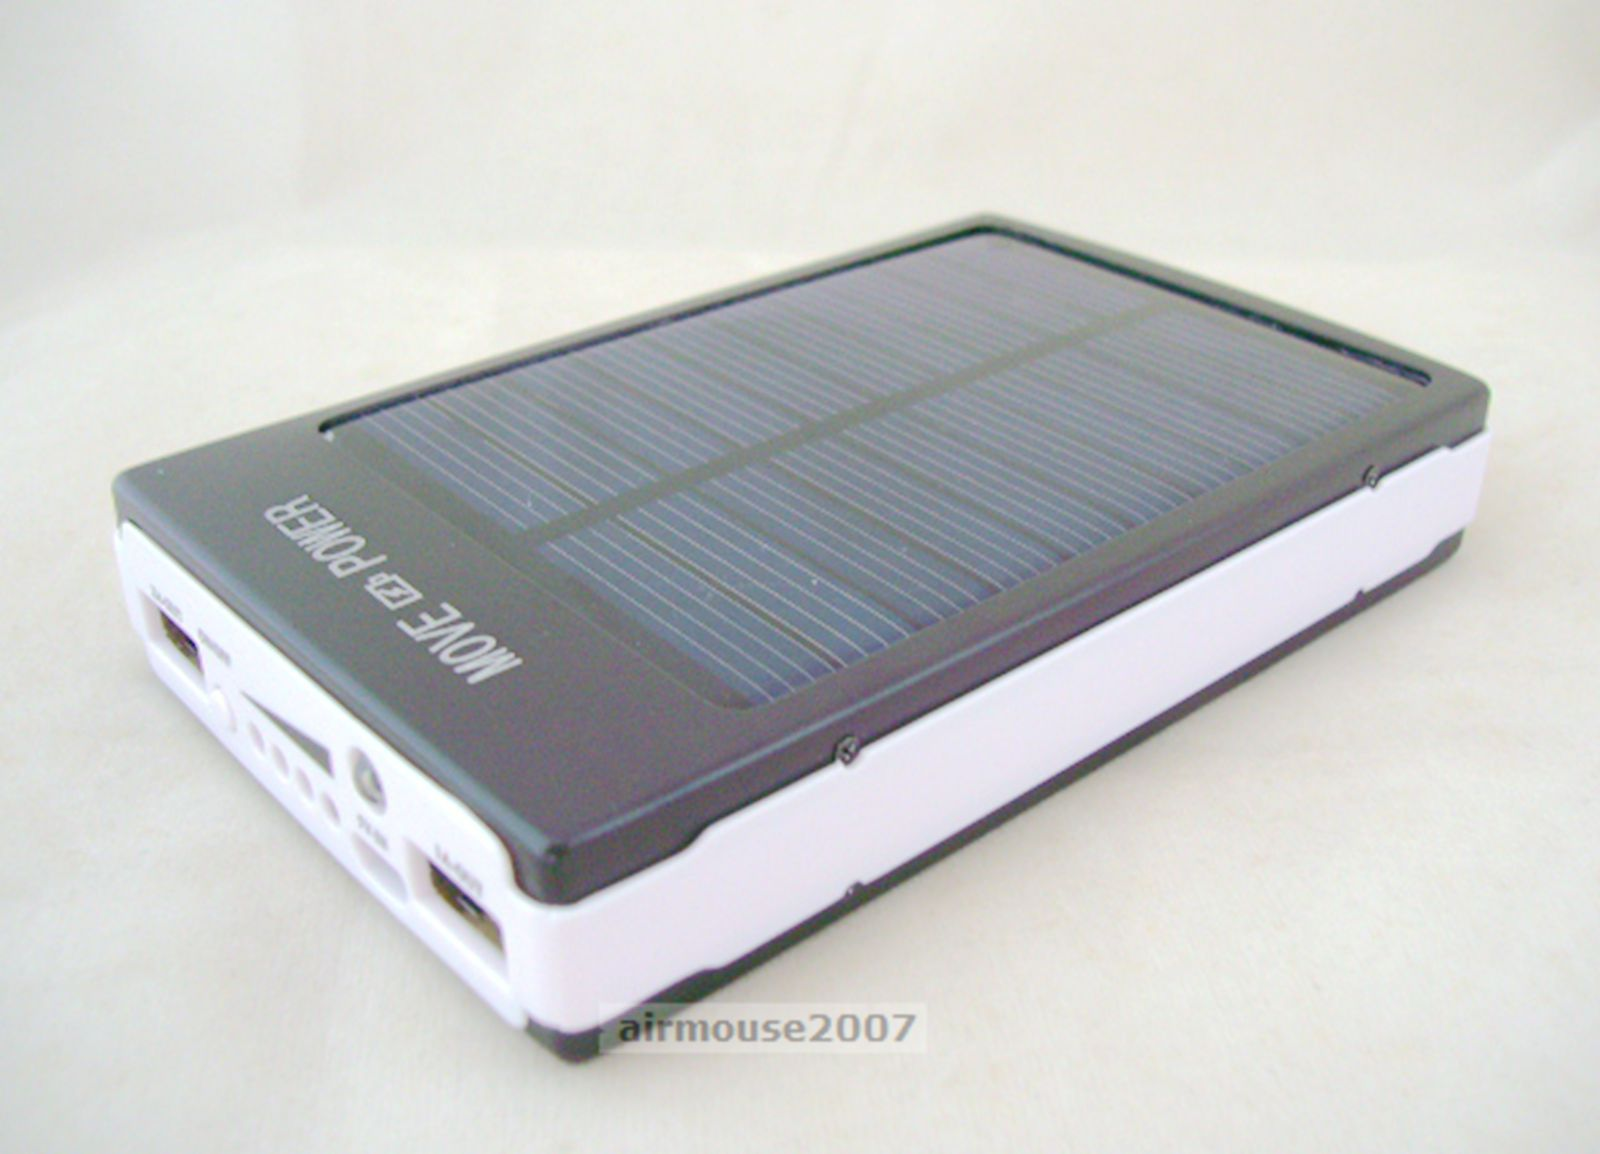
\includegraphics[width=0.5\textwidth]{bateria.jpg}
\caption{\label{fig:bateria}Bateria com fotocélula}
\end{figure}

\subsection{Sensor de temperatura e umidade}

\begin{figure}[ht!]
\centering
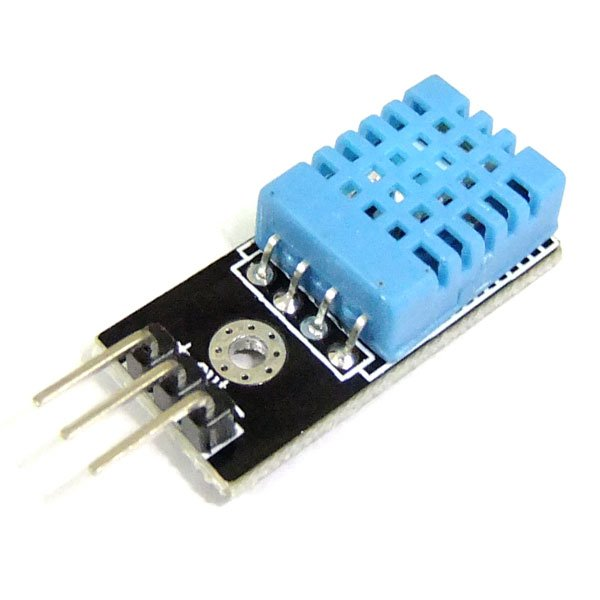
\includegraphics[width=0.5\textwidth]{dht11.jpg}
\caption{\label{fig:dht11}Sensor de temperatura e umidade}
\end{figure}

Para a medição da temperatura e da umidade do ar, será utilizado um módulo chamado DHT11, que faz a medição de temperatura e umidade do ar de forma digital.

O DHT11 é um sensor de temperatura e umidade que permite fazer leituras de temperaturas entre 0 a 50 Celsius e umidade entre 20 a 90\%, muito usado para projetos com Arduino.

O elemento sensor de temperatura é um termistor do tipo NTC e o sensor de Umidade é do tipo HR202, o circuito interno faz a leitura dos sensores e se comunica a um microcontrolador através de um sinal serial de uma via.

Alguns testes serão feitos para mensurar a corretude dos dados coletados com o sensor.

\subsection{Sensor de iluminação}

Para fazer a medição da iluminação será utilizado um resistor dependente de luz (\textit{Light Dependent Resistor}) ou LDR. O LDR é um resistor analógico cuja resistência aplicada ao circuito varia de acordo com o nível de iluminação captado, podendo assim capturar a variação da resistência e criar com isso uma tabela de equiparação com a luz, seja  solar ou artificial em diversos momentos do dia afim de tirar uma média desses valores. 

\begin{figure}[ht!]
\centering
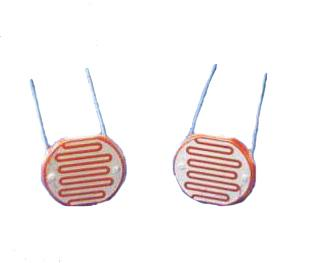
\includegraphics[width=0.3\textwidth]{ldr.jpg}
\caption{\label{fig:ldr}Sensor de luz (fotocélula)}
\end{figure}

\subsection{Sensor de som}

O nível de ruído será capturado através de um módulo de som, que consiste em um pequeno microfone com um potênciometro para regular a sensibilidade do mesmo.

O objetivo do sensor de som KY-038 é medir a intensidade sonora do ambiente ao seu redor, variando o estado de sua saída digital caso detectado um sinal sonoro. Possui um microfone de condensador elétrico e pode ser usado em sistemas de alarme por exemplo.

O limite de detecção pode ser ajustado através do potenciômetro presente no sensor que regulará a saída digital D0. Contudo para ter uma resolução melhor é possível utilizar a saída analógica A0 e conectar a um conversor analógico/digital, como a presente no Arduino por exemplo.

\begin{figure}[ht!]
\centering
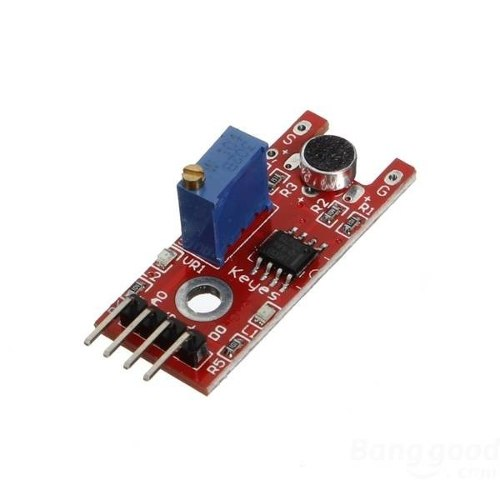
\includegraphics[width=0.5\textwidth]{som.jpg}
\caption{\label{fig:som}Sensor de som}
\end{figure}

\subsection{Acelerômetro}

O nível de trepidação será capturado através de um módulo digital de um acelerômetro de 3 eixos modelo MMA7361, fixando o eito y como nível vertical, ele capturará as variações neste eixo enquanto o dispositivo está ligado, podendo assim perceber trechos de maior variação indicando possivelmente um terreno mais acidentado e por conseguinte menos própício ao uso da bicicleta.

O MMA7361 é um módulo que possui um micro capacitor para medição do sinal sendo que o módulo possui um filtro para atenuação de ruídos e um circuito próprio para compensação da temperatura, estes conjuntos aliados formam um acelerômetro de alta sensibilidade com um baixo consumo de energia.

Existe a possibilidade de escolher entre 2 níveis de sensibilidade (1,5g / 6g). Diferente dos outros acelerômetros este já possui os terminais soldados ao dispositivo, tornado-o mais fácil e rápido o seu uso. Possui um modo de baixo consumo de energia, ideal para uso com bateria.

\begin{figure}[ht!]
\centering
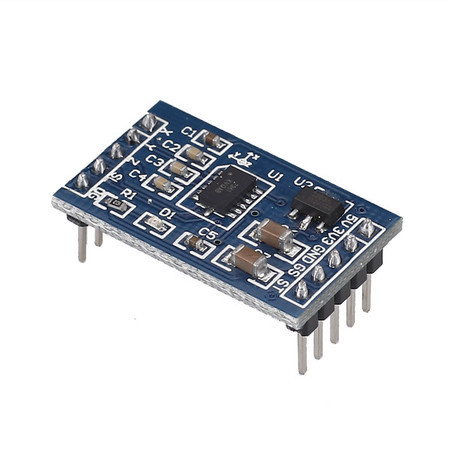
\includegraphics[width=0.5\textwidth]{acelerometro.jpg}
\caption{\label{fig:acelerometro}Acelerômetro de 3 eixos}
\end{figure}

\subsection{Geolocalizador}

A geolocalização será feita através de um \textit{shield} GPS, \textit{global positioning system}, fabricado pela empresa ITEAD Studio.

Este \textit{shield} para Arduino é um módulo GPS projetado para o receptor do Sistema de Posicionamento Global com a interface SD. Apesar de poder ser usado para armazenamento dos dados, o módulo de micro sd não será utilizado nesse projeto. Este shield pode operar com nível de tensão de operação compatível com  5V/3.3V afim de torná-lo compatível com placas Arduino e outras placas compatíveis arduino.

O shield é baseado no módulo GPS, modelo GPS REB-4216, e é compatível com as placas Arduino/MEGA. Os pinos de comunicação GPS regular (RX, TX) podem ser ligados aos pinos digitais D0-D7 do Arduino.

Ele é adequado para as seguintes aplicações com Arduíno:

\begin{itemize}
     \item Navegação Automotiva
     \item Posicionamento pessoal
     \item Gerenciamento da frota
     \item Navegação marítima
\end{itemize}

\begin{figure}[ht!]
\centering
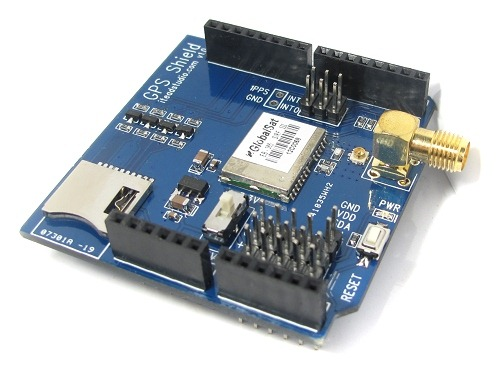
\includegraphics[width=0.5\textwidth]{gps.jpg}
\caption{\label{fig:gps}GPS Itead Studio}
\end{figure}

Este \textit{shield}  GPS possui seu próprio microcontrolador e seu \textit{software} embarcado é responsável por encontrar os satélites, fazer a conexão com os mesmos e repassar as informações recebidas através de uma conexão serial, por tanto se faz necessário criar uma conexão serial entre o \textit{shield} GPS e o Arduíno. 

\subsubsection{NMEA 0183}

O \textit{National Marine Electronics Association} (NMEA) desenvolveu uma especificação que define a interface entre diversos equipamentos eletrônicos marinhos. A norma permite que equipamentos eletrônicos marinhos possam enviar informações para os computadores e outros equipamentos marítimos.

A NMEA 0183 é um conjunto de especificações de dados e elétricas para comunicação de dispositivos eletrônicos de navegação tais como Anemômetros, ecolocalizadores, girocompassos, piloto automático, receptores GPS e muitos outros tipos de instrumentos.

Esse conjunto de especificações é necessário para decodificar as informações vindas do GPS.

Comunicação receptor GPS é definido dentro desta especificação. A maioria dos programas de computador que fornecem informações sobre a posição em tempo real entendem e esperam que os dados sejam em formato NMEA. Estes dados incluem a solução PVT completa (posição, velocidade, tempo) calculado pelo receptor de GPS. 

A idéia do NMEA é enviar uma linha de dados chamado sentença que é totalmente auto-contido e independente de outras sentenças. Existem sentenças padrões para cada categoria de dispositivo e há também a capacidade de definir sentenças proprietárias para uso pela empresa individual. Todas as sentenças padrão têm um prefixo de duas letras que definem o dispositivo que usa esse tipo de sentença, (Para os receptores GPS o prefixo é GP.) que é seguido por uma sequência de três letras que definem os conteúdos dsas sentenças. Além disso, o padrão NMEA permite que fabricantes de hardware possam definir suas próprias sentenças proprietárias para qualquer fim que entenderem. Todas as sentenças proprietárias começam com a letra P e são seguidas com 3 letras que identificam o fabricante dessa sentença. Por exemplo, uma sentença Garmin começaria com PGRM e Magellan começaria com GNPM.

Cada sentença começa com um "\$" e termina com uma sequência de retorno/fim de linha e não pode conter mais de 80 caracteres de texto visível (mais os terminadores de linha). Os dados estão contidos dentro desta linha única com itens separados por vírgulas. Os dados em si são apenas texto ASCII e podem ser estendendidos ao longo de várias sentenças em certos casos especializados, mas normalmente são totalmente contidos em uma frase comprimento variável.

Os dados podem variar na quantidade de precisão contida na mensagem. Por exemplo o tempo pode ser indicado para a parte decimal de um segundo ou a localização pode ser vista com 3 ou até 4 dígitos depois do ponto decimal. Programas que lêem os dados só devem usar as vírgulas para determinar os limites do campo e não depender das posições das colunas. Existe uma disposição para uma soma de controle no final de cada período, que pode ou não pode ser verificada pela unidade que lê os dados. O campo checksum consiste de um '*' e dois dígitos hexadecimais que representam um bit OU exclusivo de todos os caracteres entre, mas não incluindo, o '\$' e '*'. A soma de verificação é necessária em algumas sentenças.

Houveram várias mudanças no padrão, mas para o uso do gps os únicos que são susceptíveis de serem encontradas são 1.5 e 2.0 através 2.3. Estes apenas especificam algumas configurações diferentes de sentenças que podem ser peculiares às necessidades de um determinado dispositivo, portanto, os gps podem precisar de ser alterados para coincidir com os dispositivos que estão sendo interligados. 

\subsection{Sonar ultra-sônico}

\begin{figure}[ht!]
\centering
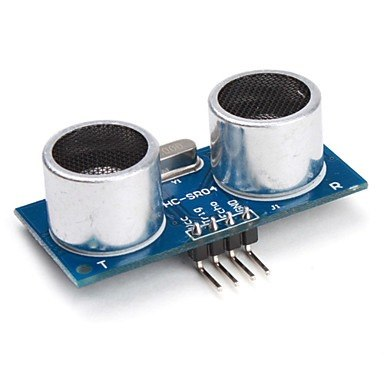
\includegraphics[width=0.5\textwidth]{ultrasom.jpg}
\caption{\label{fig:ultrasom}Sonar ultra-sônico}
\end{figure}

A distância entre um veículo motorizado e o ciclista será medida por um sensor ultra-sônico modelo HC-SR04. Este sensor emite ondas ultra-sônicas e as recebe de volta depois que as ondas são rebatidas por algum objeto, ele então calcula a distância do objeto com base na diferença do tempo entre emissão e recebimento.

O sensor ultrassônico HC-SR04 é capaz de medir distâncias de 2cm a 4m com ótima precisão. Este módulo possui um circuito pronto com emissor e receptor acoplados e 3 pinos (VCC, Trigger/ECHO, GND) para medição.

Para começar a medição é necessário alimentar o módulo e colocar o pino Trigger em nível alto por mais de 10us (microssegundos). Assim o sensor emitirá uma onda sonora que ao encontrar um obstáculo rebaterá de volta em direção ao módulo, sendo que neste tempo de emissão e recebimento do sinal o pino ECHO ficará em nivel alto. Logo o calculo da distância pode ser feito de acordo com o tempo em que o pino ECHO permaneceu em nível alto após o pino Trigger ter sido colocado em nível alto. A fórmula da distância pode ser descrita como, Distância = [Tempo ECHO em nível alto * Velocidade do Som] / 2.

A velocidade do som poder ser considerada idealmente igual a 340 m/s, logo o resultado é obtido em metros se considerado o tempo em segundos. Na fórmula a divisão por 2 deve-se ao fato que a onda é enviada e rebatida, logo ela percorre 2 vezes a distância procurada.

\section{Artefatos de software}

Como parte da solução desenvolvida, foi necessário também o desenvolvimento de alguns artefatos de \textit{software} que serão apresentados nas sub-sessões abaixo.

\subsection{Implementação no Arduíno}

A linguagem de programação adotada, oficialmente, na plataforma Arduíno, é a \textit{Arduino programming language}\cite{arduinopl} que nada mais é do que um conjunto mais restrito da linguagem C++ com algumas bibliotecas específicas.

O projeto Arduíno mantém também uma \textit{Integrated Development Environment} ou IDE, onde é possível seguir todo o fluxo de desenvolvimento para a plataforma, desde a criação de bibliotecas, codificação da aplicação, compilação da aplicação e o processo de embarcar o binário para a placa além de possuir versão para os sistemas  operacionais Windows, GNU/Linux e Mac OS X.

A escolha da linguagem se deu pela \textit{Arduino programming language}, por ela ser uma linguagem de médio nível, possuir boa documentação, uma comunidade ativa de desenvolvedores que mantém um fórum para troca de informações e por já possuir domínio com a mesma. A IDE foi escolhida foi a do próprio Arduíno, por possuir todas as ferramentas necessárias para o desenvolvimento na plataforma.

A aplicação embarcada possui 3 funcionalidades distintas, a leitura dos dados dos sensores, a formação de um arquivo JSON (\textit{JavaS
cript Object Notation} melhor explicado na seção 6.5. Armazenamento de dados) com os dados obtidos, e o envio desse JSON através da comunicação serial. Essa sequência de instruções é repetida indefinidamente desde o momento em que o dispositivo é ligado, até o momento em que o dispositivo é desligado.

\subsection{Implementações no Raspberry Pi}

A implementação feita no Raspberry Pi foi escrita em Python versão 2.7. Para ter acesso ao sistema operacional do Raspberry Pi temos algumas opções, podemos ligá-lo diretamente em um monitor, acessá-lo via rede, caso esteja conectado e possua um ip válido, e por fim usar a saída serial padrão com um adaptador USB/serial para acessá-lo pelo console do GNU/Linux.

Foi escolhida a terceira opção por praticidade em demonstrar e trabalhar com a aplicação em qualquer computador com uma entrada USB e uma aplicação para ler e escrever através da conexão serial.

Foi criado um script em Python que possui duas funções principais, a primeira interage com o banco de dados, inserindo em uma tabela um valor incremental que funciona como o identificador das medições, visto que o sistema gerenciador de banco de dados usado não suporta tal funcionalidade.

Em seguida esse script abre a conexão serial e recebe os dados, faz alguns ajustes necessários nos dados e os salva no banco de dados.

Nesta aplicação, se fez necessário a manipulação da inicialização do GNU/Linux afim de inserir esse script junto com a inicialização, para que ele não necessite que algum usuário faça login no sistema operacional e o execute.

\subsection{Licenciamento de códigos}

Os códigos desenvolvidos para este projeto estão disponibilizados numa plataforma online de versionamento colaborativa chamada \cite{github} github. O github além de ser um repositório distribuído e gratuito para projetos de software livre e código aberto, conta com uma plataforma social para que pessoas possam contribuir com os projetos nele existentes.

Todos os códigos desenvolvidos estão sobre a licensa \textit{Generel Public License} versão 3.

\subsection{Comunicação entre dispositivos}

A comunicação entre o Arduíno e o Raspberry Pi é um ponto chave do funcionamento do sistema sendo assim, um ponto de atenção e possivelmente um ponto limítrofe do mesmo.

A comunicação entre os dispositivos pode ser feita de viversas maneiras diferentes, mas todas elas possuem um ponto em comum, é necessário um terceiro \textit{hardware} para que haja a comunicação.

Inicialmente é possível apresentar duas distinções claras sobre este tipo de comunicação a depender do meio que a informação é trafegada. É possível o uso de \textit{hardwares} para  comunicação entre os dispositivos utilizando um cabo de dados, ou através de conexão sem fio. Cada uma destas modalidades pode ser novamente divididas por suas peculiaridades, apresentando vantagens os desvantagens pertinentes a cada meio e dispositivo usado.

\subsubsection{Uso de cabo de dados}

A comunicação entre o Raspberry Pi e o Arduíno feita através de meio físico pode ser feita através de cabos por onde passam as informações entre as duas placas, nesse quesito encontram-se a comunicação serial entre o GPIO do Raspberry Pi e os pinos seriais do Arduíno, a comunicação serial entre os pinos I2C do Raspberry Pi e os pinos seriais  do Arduíno, e por fim o uso do cabo USB entre as saídas USB dos dois dispositivos.

Para utilizar a comunicação através de meio físico dos dispositivos é necessário ter alguns cuidados e se atentar a alguns pontos. Os pinos I2C trabalham com uma voltagem diferente dos pinos seriais do Raspberry Pi, por isso, se faz necessário utilizar um circuito divisor de voltagem. Além disso, O Raspberry Pi não possui uma bilbioteca nativa para trabalhar com conexões seriais, para isso precisamos utilizar uma biblioteca de alto nível para a linguagem escolhida.

Para o projeto Bduíno, foi escolhido o método mais simples de comunicação, a comunicação através da USB usando uma bilbioteca de abstração de comunicação serial da própria linguagem, a PySerial do Python2. Além do trafego de dados, a conexão com cabo USB, encarrega-se também da alimentação elétriva do Arduíno através da porta USB do Raspberry Pi.

\subsubsection{Conexão sem fio}

Para a comunicação sem fio é necessário o uso de outros \texttt{hardwares} de comunicação, duas das opções disponíveis são o uso de rádio frequência e o uso de bluetooth. Em ambos os casos, há uma dependência de \textit{hardware} em ambas as pontas da comunicação, esses hardwares fazem a transmissão e recepção dos dados usando ondas como meio de propagação. 

As duas tecnologias são bastante usadas, a radiofrequência possui um uso mais amplo, mas por trabalhar com frequencias de ondas usadas por muitos tipos de aparelhos, pode ocorrer interferências na comunicação, com o bluetooth, a comunicação é feita através de um canal previamente criado e autorizado entre dois dispositivos, deixando assim a comunicação mais confiável, entretanto a necessidade da comunicação e configuração inicial pode se mostra um ponto negativo a se considerar.

\subsection{Armazenamento de dados}

Para o armazenamento de dados foi feito um estudo e um teste de desempenho entre duas tecnologias amplamente utilizadas para armazenamento de dados, a \textit{eXtensible Markup Language} ou XML e o \textit{JavaScript Object Notation} ou JSON. As duas tecnologias armazenam os dados em um arquivo de texto plano, mas possuem diferenças que trazem características únicas a cada um deles.

Os testes incluíam testes de leitura, gravação e tráfego de dados entre o Arduíno e o Raspberry Pi. Tendo o JSON uma vantagem em relação ao XML, sendo então escolhido o JSON como formato padrão.

Depois dos dados serem recebidos no Raspberry Pi, eles são gravados em um sistema gerenciador de banco de dados chamado SQLite. 

O SQLite foi escolhido por ser amplamente utilizado em sistemas embarcados, por seu tamanho e facilidade de uso. O Sqlite possui algumas limitações inerentes, como a inexistência de relacionamentos entre as tabelas, por isso uma simulação de \textit{software} se fez necessária. O modelo de dados é bem enxuto e grava apenas um numero incremental que armazena o identificador da atividade, a data e hora de cada checagem, e os dados armazenos em formato JSON.

\begin{figure}[ht!]
\centering
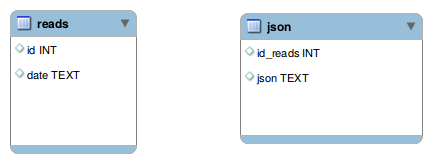
\includegraphics[width=0.5\textwidth]{db.png}
\caption{\label{fig:db}Diagrama de dados}
\end{figure}

Não existe relacionamento entre as tabelas pois este recurso é inexistente no sistema gerenciador de banco de dados, mas um tipo de relacionamento lógico foi criado através da aplicação.

\subsection{Arquitetura da aplicação}

\begin{figure}[ht!]
\centering
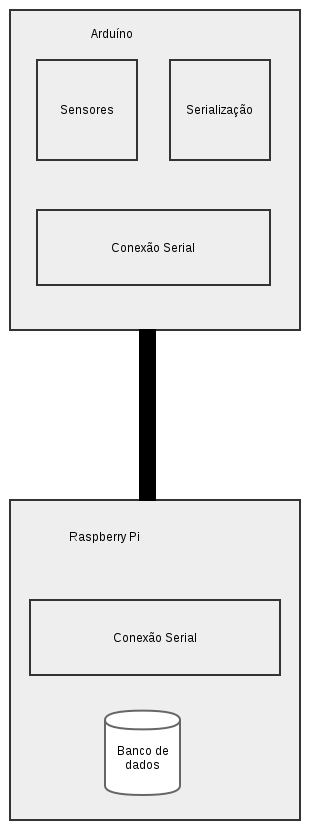
\includegraphics[width=0.3\textwidth]{deployment.png}
\caption{\label{fig:mega}Diagrama de implantação}
\end{figure}

A arquitetura da alicação é naturalmente distribuída, pela natureza da solução construída, por isso foi utilizado uma arquitetura em camadas, onde a camada mais inferior só recebe os dados da camada superior, mas não retorna nenhuma informação para ela. O conector usado entre as camadas é o fluxo ou \textit{stream}.

A figura 16: Diagrama de implantação é uma imagem representativa da arquitetura pretendida, afim de ilustração.

Por questão de desempenho e melhor aproveitamento de recursos, a aplicação não está dividida em módulos, para este fim , as funções servem como tal.

\section{Testes e resultados}

Os testes foram feitos com o protótipo em ambiente urbano, em sessões de aproximadamente 30 minutos, por localidades diversas na cidade de Salvador.

\begin{figure}[ht!]
\centering
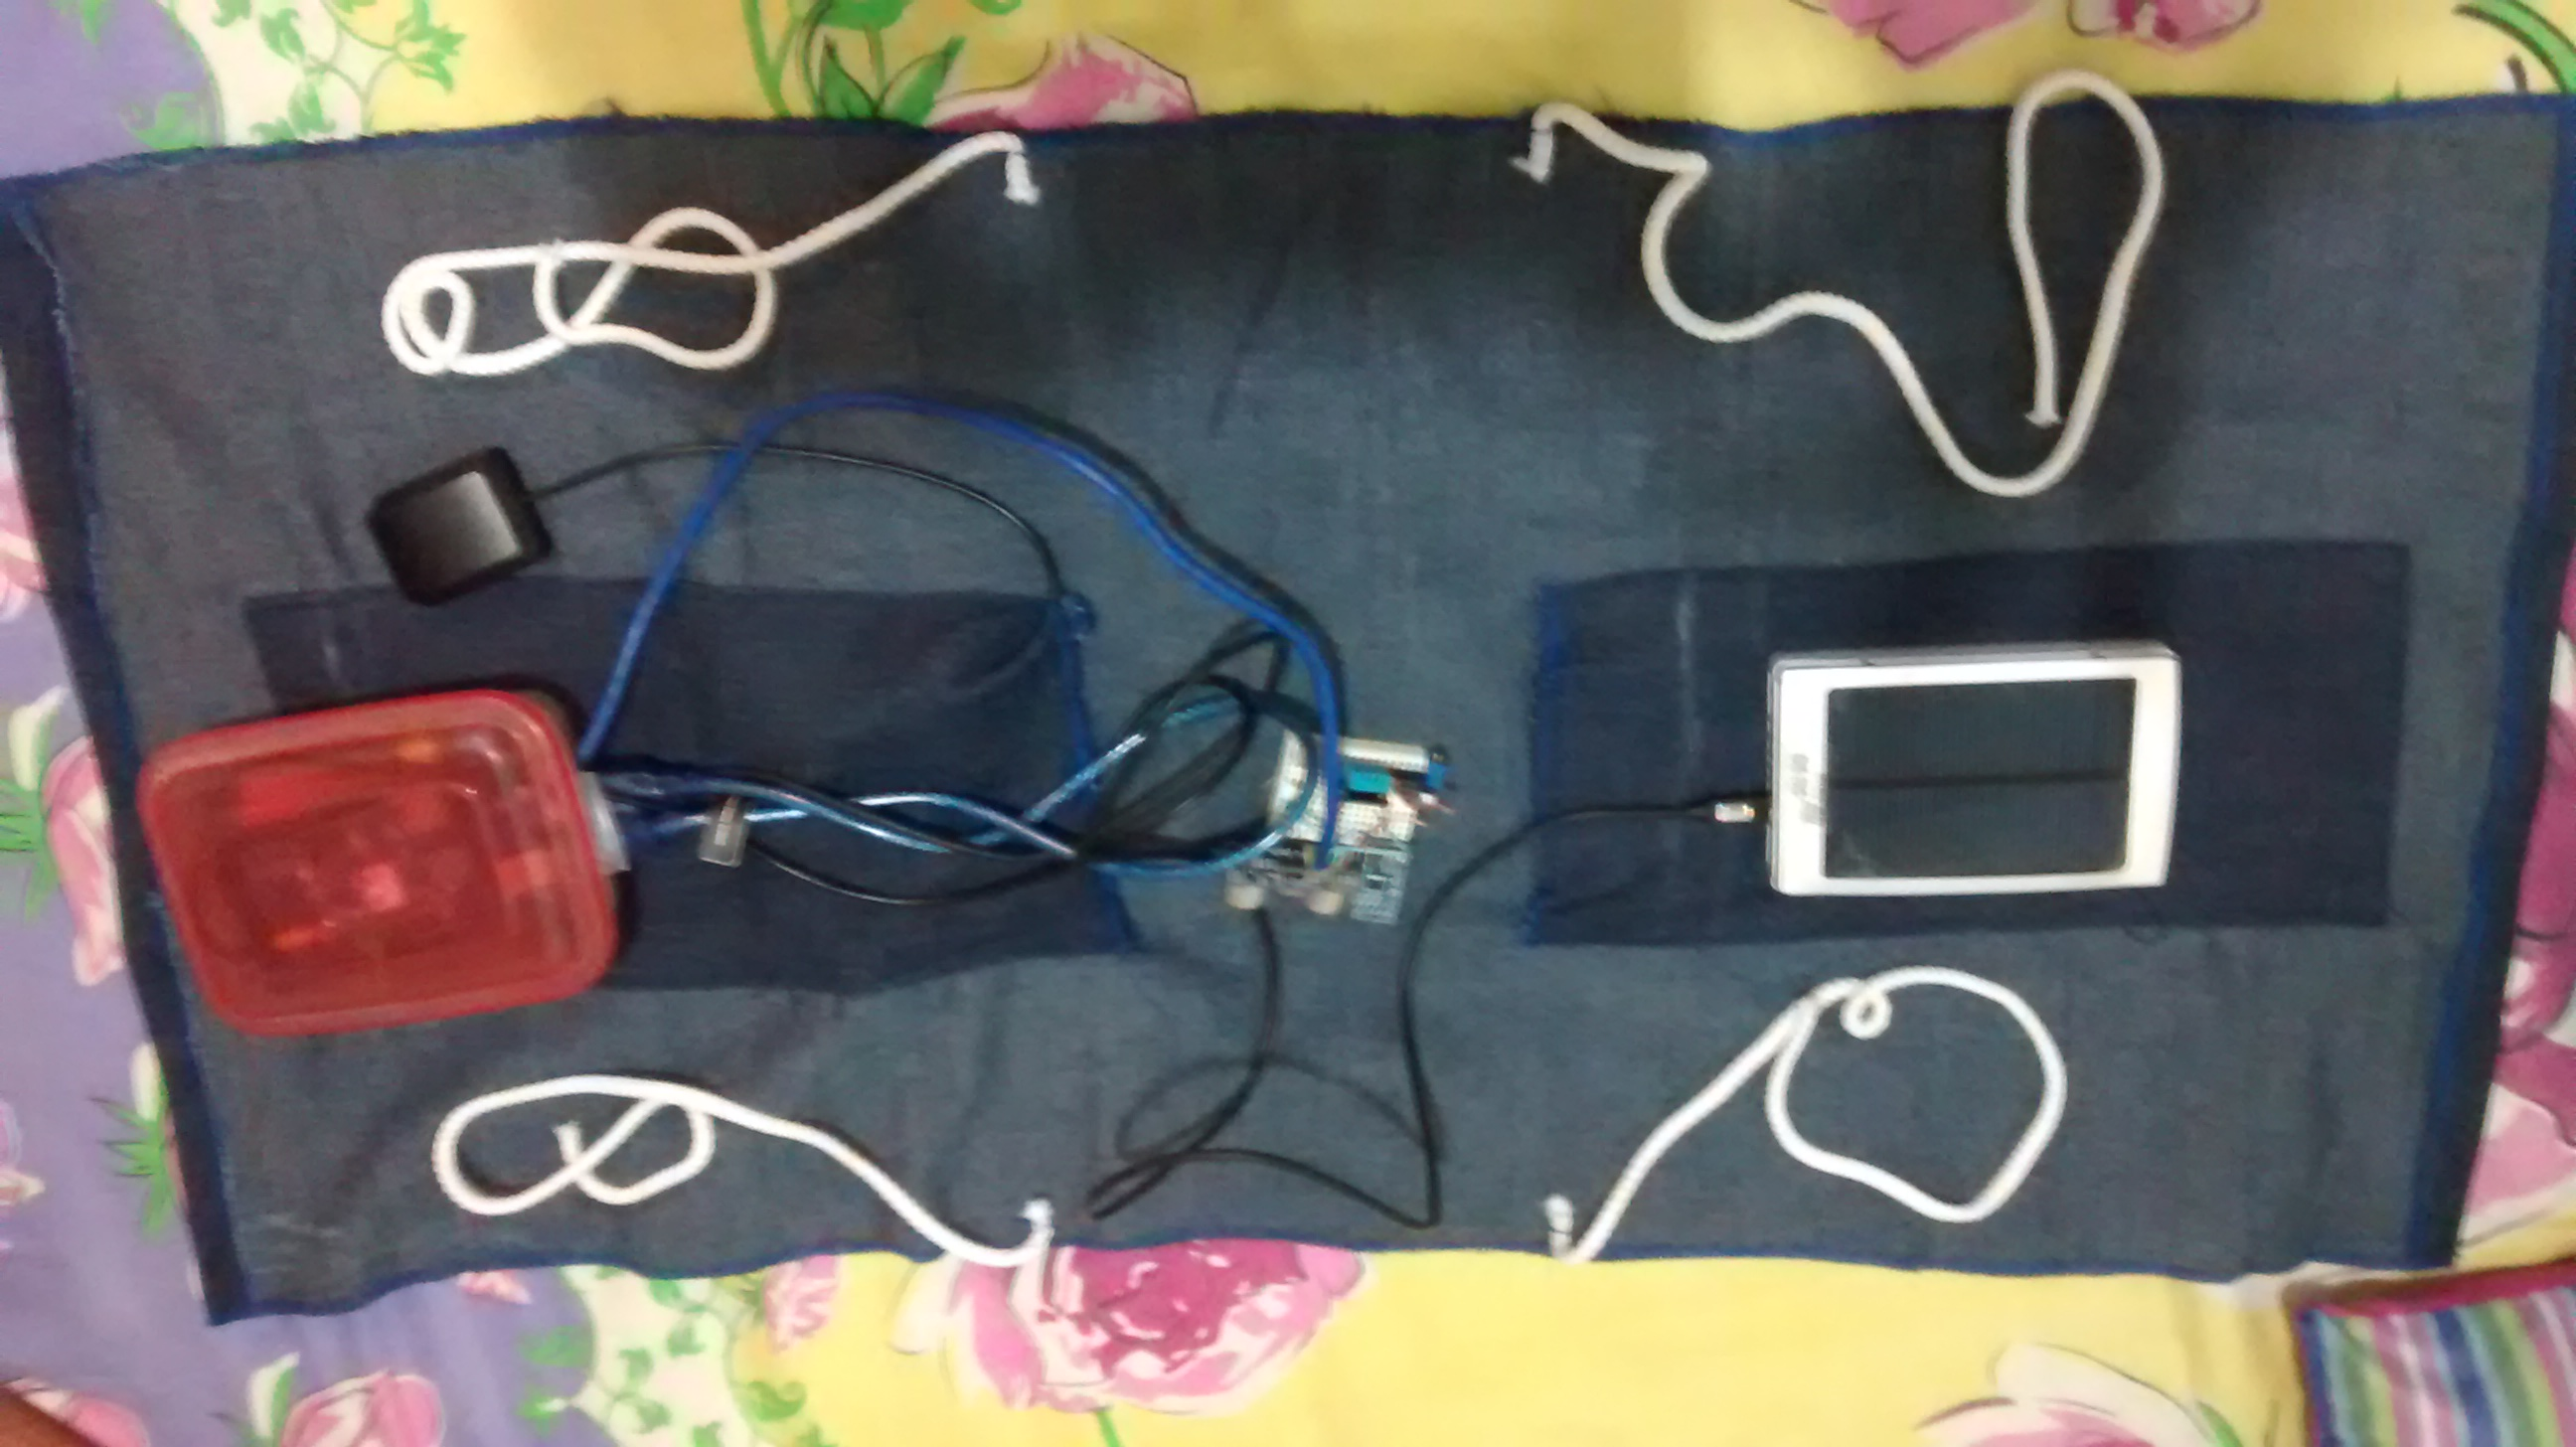
\includegraphics[width=0.5\textwidth]{prototipo.jpg}
\caption{\label{fig:prototipo}Protótipo do dispositivo}
\end{figure}

Este protótipo é montado numa bolsa de tecido a qual dobra-se ao meio no quadro ou na garupa da bicicleta, e conta com dois cordões para dar sustentação e equilíbrio..

O teste contou com dois ciclistas voluntários para o mesmo.

Após os dados coletados, foi possível a manipulação e leitura dos  dados coletados afim de uma análise inicial. Esta primeira análise, apesar de possuir os dados completos de todos os sensores, levou em consideração apenas um fator mensurado, a distância que o veículo passa por uma bicicleta, para a criação destes gráficos. 

De acordo com o artigo 201 do código de trânsito brasileiro - CTB a distância mínima segura ao ciclista é de 1,5 metros ao fazer uma ultrapassagem.

Foram criados dois gráficos, ilustrando o resultados das medições efetuadas. O primeiro gráfico mostra a relação entre o número de veículos aproximados que ultrapassam o ciclista, pela distância que eles o fazem em uma determinada medição (900 pontos analisados):

Uma medição é feita apartir da leitura dos dados de um determinado ponto em sua trajetória. Cada medição relativa a distância pode variar entre os objetos que passam pela bicicleta, como um carro, um ônibus, ou mesmo nenhum objeto. 

\begin{figure}[ht!]
\centering
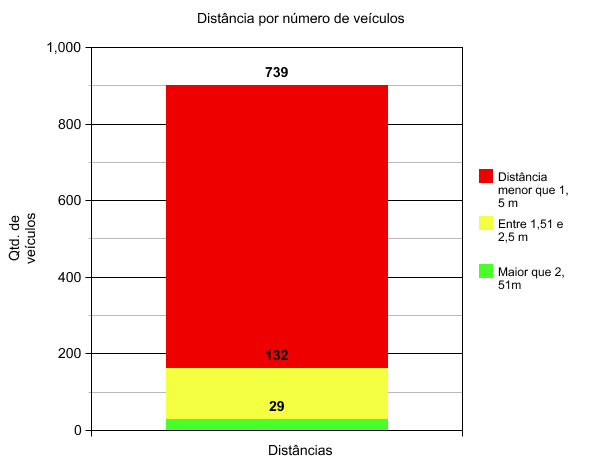
\includegraphics[width=0.5\textwidth]{graph1.png}
\caption{\label{fig:graph1}Gráfico de distância por quantidade de veículos em uma medição}
\end{figure}

O segundo gráfico exibe a mesma relação do gráfico anterior, mas totalizando as 06 medições efetuadas (5400 pontos analisados).

\begin{figure}[ht!]
\centering
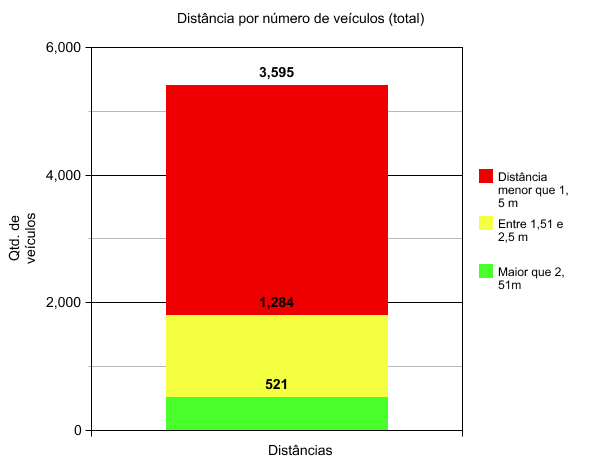
\includegraphics[width=0.5\textwidth]{graph2.png}
\caption{\label{fig:graph2}Gráfico de distância por quantidade de veículos totais}
\end{figure}

\section{Conclusão}

Ao final do projeto, o dispositivo criado suportou as operações pensadas em sua concepção, ele consegue medir os valores de sensores diversos, armazenando num sistema gerenciador de banco de dados com exeção citada anteriormente. O Bduíno foi capaz de capturar dados ambientais e do contexto urbano para responder questões sobre mobilidade urbana, inspirado numa demanda global, adaptada para um contexto local, facilmente replicável e modificável.

\section{Trabalhos futuros}

Sendo esta solução de código aberto e flexível, é possível que o trabalho seja expandido no futuro com novas melhorias e funcionalidades, tais como:

\begin{itemize}

  \item Envio de dados no momento da coleta para um servidor.
  \item Adição de um novo sensor de gás carbônico.
  \item Melhorar o cálculo de velocidade de veículos motorizados.
  \item Utilizar também um dînamo para coletar energia mesmo pedalando em ambientes pouco iluminados.
  \item Criação de uma plataforma para visualização dos dados.
  \item O Uso de threads para tratar operações críticas como acesso a banco e leitura de dados na comunicação serial.
  
Algumas das modificações para o futuro podem ser facilmente implementadas, outras demandam maior esforço e podem representar outros trabalhos.

No início do projeto foi pensado na possibilidade do uso do sensor ultrasônico, HC-SR04 para medir a velocidade que um carro passa por uma bicicleta, essa medição se tornou inviável por uma série de motivos diferentes, dentre eles: 

\begin{itemize}
\item O tipo de sensor usado emite suas ondas ultra-sônicas em propagação cônica, ao invés de linear, tendo assim mais tempo de captura de dados da mesma fonte, diminuindo o intervalo de cálculo.

\item O sistema existente tende a estar em movimento no mesmo sentido e direção da fonte calculada, necessitando-se assim do cálculo da velocidade média do sistema, que hoje não é possível com módulo atual.
\end{itemize}

Para esta funcionalidade se faz necessário um pouco mais de pesquisa e um equipamento mais especializado.


\end{itemize}

\bibliographystyle{model1-num-names}
%\bibliography{acmtog-sample-bibfile}

\section{Referências}
\begin{thebibliography}{00}

  \bibitem{Arduino}
  Arduíno Introduction, disponível em \url{http://www.arduino.cc/en/Guide/Introduction}. Ultimo acesso em 26/05/2014.
  \bibitem{marshallbrainmicrocontrolador}
  O que é um microcontrolador, disponível em \url{http://tecnologia.hsw.uol.com.br/microcontroladores1.htm}. Último acesso em 10/01/2015.
  \bibitem{Wikihouse}
  Wikihouse, disponivel em \url{http://www.wikihouse.cc/}. Ultimo acesso em 26/05/2014.
   \bibitem{Open Source Ecology}
   Open Source Ecology, disponível em \url{http://opensourceecology.org/}. Último acesso em 26/05/2014.
   \bibitem{Machines: Global Village Construction Set}
   Machines: Global Village Construction Set, disponivel em \url{http://opensourceecology.org/gvcs/}. Último acesso em 26/05/2014.
   \bibitem{Arc e Tec}
   Arc e Tec, disponível em \url{http://www.arq-e-tec.com/2011/09/wikihouse-projetos-de-arquitetura-open-source/}. Último acesso em 26/05/2014.
   \bibitem{softwareLivre}
   Free Software Foundation, disponível em \url{https://www.fsf.org/about/what-is-free-software}. Último acesso em 10/01/2015.
   \bibitem{GNU}
   GNU Operating System, disponível em \url{http://www.gnu.org/}. Último acesso em 10/01/2015.
   \bibitem{e-bikes}
   Electric bikes start to come of age, disponível em \url{http://www.bikeradar.com/news/article/electric-bikes-start-to-come-of-age--18203/}. Último acesso em 10/01/2015.
   \bibitem{Conexao Serial}
   The RS232 Standard, disponível em \url{http://www.camiresearch.com/Data_Com_Basics/RS232_standard.html}. Último acesso em 10/01/2015.
   \bibitem{Raspberry Pi}
   What is a Raspberry Pi?, disponível em \url{http://www.raspberrypi.org/help/what-is-a-raspberry-pi/}.
   Último acesso em 10/01/2015.
   \bibitem{tecnologia verde}
   FERREIRA, Alisson Gonçalves. \emph{Tecnologias da informação verdes.}. 2009. 29 f. Trabalho de conclusão de curso (Especialização em Ecologia humana) - Instituto Superior de Educação do Paraná, Maringá, 2009. [Orientador: Fábio Angeoletto.]
   \bibitem{arduinopl}
   Language Reference, disponível em \url{http://arduino.cc/en/Reference/HomePage}. Último acesso em 10/01/2015.
   \bibitem{github}
   Github, disponível em \url{https://github.com/about}.
   Último acesso em 10/01/2015.
   \bibitem{SolarFuel}
   Solar Fuels and Artificial Photosynthesis, disponível em 
   \url{http://www.rsc.org/campaigning-outreach/global-challenges/energy/}. Último acesso em 10/01/2015.
   \bibitem{pesquisamobilidade}
   Pesquisa de mobilidade, disponível em \url{http://www.seinfra.ba.gov.br/mobilidade2012/mobilidade.html}. Último acesso em 10/01/2015.
   \bibitem{pythonsite}
   About Python, disponível em \url{https://www.python.org/about/}. Último acesso em 10/01/2015.
   \bibitem{artigoenergiasolar}
   International Energy Agency (2011)
   \bibitem{programandoraspberrypi}
   S. Monk, Programando o Raspberry Pi, primeiros passos com Python, novatec, 2013.
   \bibitem{arduinoworkshop}
   J. Boxall, Arduino workshop A hands-on introduction with 65 projects, No Starch Press, 2013.
   \bibitem{artigotcw}
   C. Outram, C. Ratti, A. Biderman, The Copenhagen Wheel: An innovative electric bicycle system that harnesses the power of real-time information and crowd sourcing, COP15 United Nations Climate Change Conference in Copenhagen, 2010.
   \bibitem{artigosensorium}
   K. Brunet, T. Oliveria, Arte, DIY e Comunicação Ambiental: Estudo de caso do projeto Sensorium, do mar para o rio, 2º Encontro Interdisciplinar de Comunicação Ambiental (EICA), 2013.
\end{document}